\documentclass{article}
\usepackage[a4paper, left=0.7in, right=0.7in, top=0.7in, bottom=0.7in]{geometry}
\usepackage{color}
\usepackage{hyperref}
\hypersetup{colorlinks=true, linktoc=all, linkcolor=blue, urlcolor=blue}
\setlength{\parindent}{0pt}
\setlength{\parskip}{1em}
\usepackage[english]{babel}
\usepackage{titlesec}
\titlespacing{\section}{0pt}{10pt plus 4pt minus 2pt}{-4pt plus 2pt minus 2pt}
\titlespacing{\subsection}{0pt}{-4pt plus 2pt minus 2pt}{-4pt plus 2pt minus 2pt}
\titlespacing{\subsubsection}{0pt}{-4pt plus 2pt minus 2pt}{-4pt plus 2pt minus 2pt}
\usepackage{bm}
\usepackage{enumitem}
\setlist[itemize]{topsep=0pt}
\setlist[enumerate]{topsep=0pt}
\usepackage{amssymb, amsthm}
\usepackage{mathtools}
\usepackage{float}
\usepackage{array}
\usepackage{graphicx}
\usepackage[capitalise]{cleveref} % must be after amsmath and hyperref
\usepackage[justification=centering]{caption}
\graphicspath{ {images/} {../fig} }
%%%%%%%%%%%%%%%% Document %%%%%%%%%%%%%%%%
\begin{document}
\begin{center}
  {\huge \underline{A Remeshing Approach to Multiresolution Modeling}} \\ \vspace{1em}
  
  {\Large {Mario Botsch \quad Leif Kobbelt}} \\ \vspace{1em}
  {A Report by: Amir Mann, Ehud Gordon}
\end{center}
\section{Introduction}
Remeshing involves modifying an existing mesh so to improve its quality and structure. Specifically, it aims to make the faces and edges more regular, both in their area and valence. This modification shouldn't change the geometry of the underlying mesh too much.

One important use of remeshing is related to the descretized Laplacian. Solving Linear systems using the discretized Laplacian is a common task in Digital Geometry Processing. The efficiency and robustness of solvers on those systems rely on the input Laplacian matrix. On symmetric matrices, these solvers achieve better results. However, for a general triangle meshes, the Laplacian matrix $L$ isn't guaranteed to be symmetric. This can be seen in \cref{eq:laplacian_ij}:
\begin{equation} \label{eq:laplacian_ij}
  L_{i,j} =  \frac{\cot \alpha_{i} + \cot \beta_{i}} {A(v_i)} \quad \quad i \neq j  
\end{equation}
where $\alpha_{i}, \beta_{i}$ are the angles of the adjacent triangles, and $A(v_i)$ is the Voronoi area of vertex $v_i$, as shown in~\cref{fig:laplaceCot2} 
\begin{figure}[H] \centering 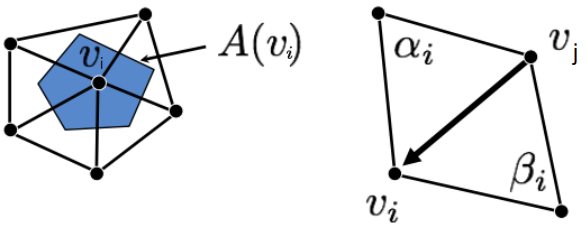
\includegraphics[height=0.3\textheight,width=0.4\textwidth,keepaspectratio]{laplaceCot2} \caption{} \label{fig:laplaceCot2} \end{figure}
Specifically, we notice that if  $A(v_i) \neq A(v_j)$, then $L_{i,j} \neq L_{j,i}$, making the resulting Laplacian unsymmetric. 

However, if we apply remeshing, thus equalizing the vertices area, we can turn $L$ into (nearly) a symmetric matrix, and use faster, more robust linear solvers.
\section{Previous Work}

\section{Algorithm}

\section{Results}

\section{Discussion}




\end{document}

